\documentclass[final]{beamer}

% beamerposter -----------------------------------------------------------------
%% 36in x 48in = 91.44cm x 121.92
\usepackage[size=custom,width=121.92,height=91.44,scale=1.0]{beamerposter}
\usetheme{gemini}
\usecolortheme{mit}

% Columns ----------------------------------------------------------------------
% % If you have N columns, choose \sepwidth and \colwidth such that
% % (N+1)*\sepwidth + N*\colwidth = \paperwidth
\newlength{\sepwidth}
\newlength{\colwidth}
\newlength{\padwidth}
\setlength{\sepwidth}{ 1.40cm}
\setlength{\colwidth}{28.00cm}
\setlength{\padwidth}{ 2.92cm}

\newcommand{\separatorcolumn}{\begin{column}{\sepwidth}\end{column}}

\setbeamertemplate{footline}[text line]{%
  \begin{beamercolorbox}[colsep*=0ex,center]{block body}
    \vskip2ex
    \normalsize{March 10th, 2023 -- Santa Fe, NM
      \hfill Conference on Data Analysis 2023}
    \vskip2ex
  \end{beamercolorbox}
}%

\title{Automatic Relevance Determination
  for Gaussian Processes with Functional Inputs}

\author{
  \textbf{Luis Damiano}\inst{1},
  Margaret Johnson\inst{2}, Joaquim Teixeira\inst{2},
  Max D. Morris\inst{3},
  Jarad Niemi\inst{1}}

\institute[Iowa State]{
  \inst{1} Department of Statistics, Iowa State University
  \inst{2} Jet Propulsion Laboratory, California Institute of Technology
  \inst{3} Departments of Statistics, and Industrial and Manufacturing
Systems Engineering, Iowa State University}

\usepackage{lipsum}\usepackage[base]{babel} % need to go together
\newcommand{\shortlipsum}{{\color{gray!99} \lipsum[1][1-10]}}

%%
\RequirePackage{tabularray}
\UseTblrLibrary{booktabs}
\UseTblrLibrary{functional} %% Enables evaluate
\NewColumnType{R}{X[r]}
\usepackage{soul}
\setul{.35ex}{.25ex}

%% Math packages
\RequirePackage{amssymb}
\RequirePackage{amsmath}
\RequirePackage{amsthm}
\RequirePackage{mathtools} % provides: coloneqq
\RequirePackage{bm}
\DeclareMathOperator*{\argmax}{arg\,max}
\newcommand{\norm}[1]{\left\lVert#1\right\rVert}
\DeclareMathOperator{\evsym}{E}
\newcommand\EE[1]{\evsym\left\langle#1\right\rangle}
\DeclareMathOperator{\vsym}{V}
\newcommand\VV[1]{\vsym\left\langle#1\right\rangle}

%% Citations
%%% Use biblatex
\usepackage[
    backend=bibtex,            % Use legacy bibtex backend (biber is better)
    natbib=true,               % Load aliases for citation commands
    citestyle=numeric-comp,    % Inline: Author year, compressed
    maxcitenames=1,            % Inline: max 1 author name
    bibstyle=authoryear,       % Bibliography: Author year
    giveninits=true,           % Bibliography: first and middle name initials
    dashed=false,              % Bibliography: no dash for recurrent authors
    abbreviate=true,           % Bibliography: abbreviate
    maxbibnames=100,           % Bibliography: all author names
    sorting=nyt,               % Bibliography: sort by name, year, title
    isbn=true,                 % Bibliography: print ISBN
    url=false,                 % Bibliography: don't print URL
    doi=true,                  % Bibliography: print DOI
    eprint=false               % Bibliography: don't print eprint information,
    ]{biblatex}
%%% bibliography: print authors as "last name, first name"
%    \DeclareNameAlias{sortname}{family-given}
%%% Add bib files
    \addbibresource{references.bib}
    \addbibresource{referencesR.bib}
\csappto{blx@filehook@postload@numeric.bbx}{%
\mode<presentation>{%
\setbeamertemplate{bibliography item}{%
\insertbiblabel}}}
%% \begin{minipage}[position][height][inner-pos]{width}

\begin{document}

\begin{frame}[t]

  \colorbox{pink}{
    \begin{minipage}[t][76cm][t]{58cm}
      \colorbox{yellow}{
        \begin{minipage}[t][20cm][t]{28cm}
          Left
          \begin{block}{Automatic Dynamic Relevance Determination}
            A framework for Gaussian Processes with functional inputs
            $X(t)\in\mathcal{X} = \left\{X:[0,1]\to\mathbb{R}\right\}$, $t\in[0, 1]$
            and a scalar output $y\in\mathbb{R}$. Let $f:\mathcal{X}\to\mathcal{Y}$ be
            an unknown function with evaluations $y_i = f(X_i)$, $i = 1, \dots,
            N\in\mathbb{N}$.
            \begin{align}
              \mathbf{y}
              &\sim \mathcal{N}\left(\mathbf{m}_f, \sigma_{f}^{2} \ \mathbf{R}_f
                + \sigma_{\varepsilon}^{2}\mathbf{I}\right) \\
              {(\mathbf{m}_f)}_i
              &= m_f(X_i) \\
              {\left(\mathbf{R}_f\right)}_{ij}
              &=
                \text{exp}\left\{
                -0.5 \phi^{-2} \ d_f(X_i, X_j)
                \right\}
              \\
              d_f(X_i, X_j)
              &= \int_{\mathcal{T}}
                \omega(t)
                {\left(X_i(t) - X_j(t) \right)}^2 dt
              \\
              \omega(t)
              &: \mathcal{T}\to\mathbb{R}^+
            \end{align}
            $\sigma_{\varepsilon}^2 > 0$,
            $\sigma_{f}^2 > 0$,
            $\phi > 0$,
            $i, j = 1, \dots, N$,
            and $m_f(\cdot)$ is a mean function left unspecified w.l.o.g.
          \end{block}

          \begin{block}{Choice of weight function}
            \begin{description}
            \item Learn how the input predictive relevance
              varies over the index space
            \item[Smoothness] Enforce smoothness on relevance
              over the index space
            \item[Parsimony] Fewer parameters than the vector representation
            \item[Interpretation]: for modeling feedback loop and
              physical model understanding
            \end{description}
          \end{block}

          \begin{block}{Learning \& validation}
            Fully Bayesian inference on the unknown quantities $\bm{\theta}$.
            One MCMC chain~\citep{raftery1992} with $M \in \mathbb{N}$ post warm-up
            samples generated via the NUTS algorithm~\citep{hoffman2014}.
            \begin{align}
              \label{eq:margina-likelihood}
              \log p(\mathbf{y} | \mathbf{X}, \bm{\theta})
              =& -\frac{1}{2}
                 {(\mathbf{y} - \mathbf{m}_y)}^\top
                 {\mathbf{S}_y}^{-1}
                 {(\mathbf{y} - \mathbf{m}_y)}
                 -\frac{1}{2}
                 \log | \mathbf{S}_y |
                 - \frac{n}{2} \log 2\pi \\
              \label{eq:parameter-posterior}
              \log p(\bm{\theta} | \mathbf{y}, \mathbf{X})
              \propto&
                       \log p(\mathbf{y} | \mathbf{X}, \bm{\theta}) +
                       \log p(\bm{\theta}).
            \end{align}

            Validation statistic posterior expectation approximated using a thinned
            posterior parameter sample with $\tilde{M} \in \mathbb{N}$ draws.
            \begin{align}
              \hat{v}_1
              &= {\tilde{M}}^{-1} \sum_{{\tilde{m}}=1}^{{\tilde{M}}} N^{-\frac{1}{2}} \norm{%
                \EE{\bm{y}_{*} | \bm{X}, \bm{X}_{*}, \bm{y}, {\bm{\theta}}_{{\tilde{m}}}} -
                \bm{y}_{*}
                } \label{eq:validation-rmse} \\
              \hat{v}_2
              &= {\tilde{M}}^{-1} \sum_{{\tilde{m}}=1}^{{\tilde{M}}}
                p(\bm{y}_{*} | \bm{X}, \bm{X}_{*}, \bm{y},
                {\bm{\theta}}_{{\tilde{m}}}) \label{eq:validation-ppld}
            \end{align}
          \end{block}

        \end{minipage}
      }
      \colorbox{green}{
        \begin{minipage}[t][20cm][t]{28cm}
          Right
          \begin{block}{Microwave Limb Sounder}
            \begin{itemize}
            \item Computer model: forward
              model~\cite{read2006,schwartz2006,waters2006} estimates, or
              \emph{retrieves}, geophysical variables from electromagnetic radiation
            \item Planetwide, daily data products~\cite{liversey2020} and uncertainty
              experiments~\cite{turmon2019,braverman2021} rely on a myriad of runs
            \item Output: score for reflected sunlight around 190GHz~\cite{johnson2020}
            \item Functional input: atmospheric profiles over a vertical grid
            \item We consider some species in pressure regions expected to be
              well-informed by the measurements~\cite{liversey2020}
            \end{itemize}
          \end{block}
        \end{minipage}
      }
      \vskip1cm
      \colorbox{yellow!33}{
        \begin{minipage}[t][50cm][t]{58cm}
          Data
          \begin{block}{Data}
            \begin{figure}
              \centering
              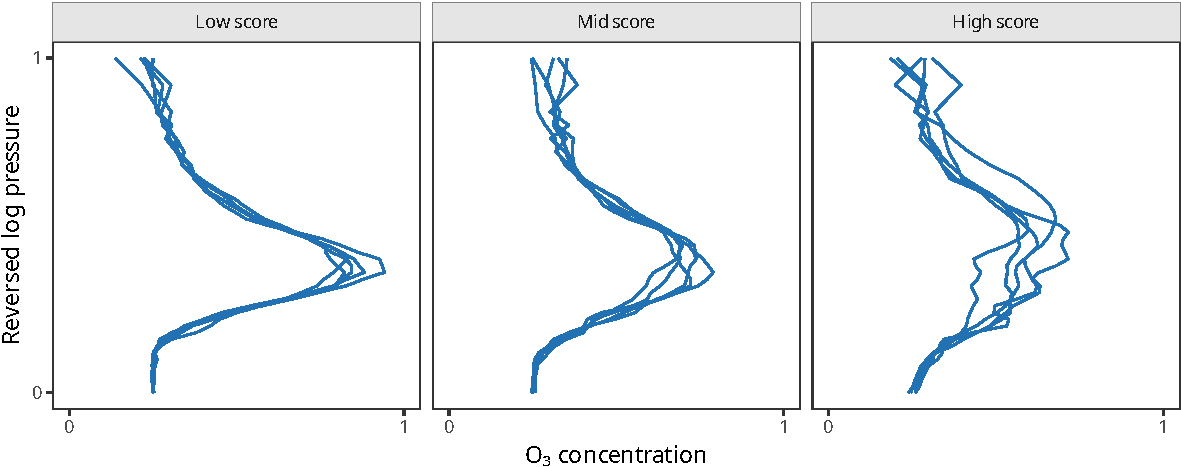
\includegraphics[width=.85\linewidth]{inc/mls_input_profiles}
            \end{figure}

            \begin{center}
              Radiance score variability seems associated with the tropopause Ozone
              concentration
            \end{center}
          \end{block}

          \begin{block}{Asymmetric Double Exponential weight function}
            \begin{figure}
              \centering
              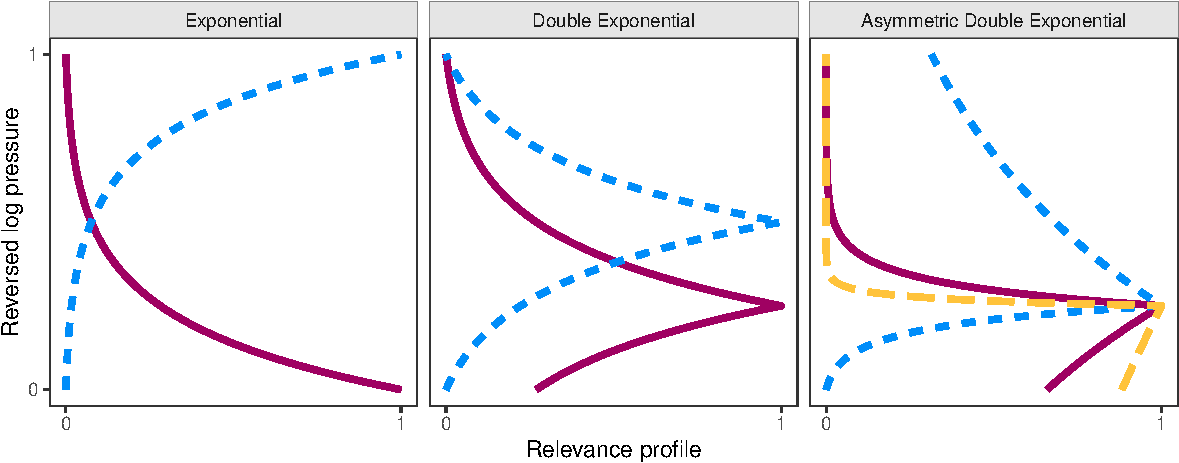
\includegraphics[width=.85\linewidth]{inc/mls_weight_profiles}
            \end{figure}

            \begin{equation}
              \omega(t)
              =
              \text{exp}\left\{-(t - \tau)\lambda\kappa^s s\right\}
            \end{equation}
            Space:
            $\omega(t): \mathcal{T} = [0, 1] \to (0, 1]$,
            $s = \text{sign}(t - \tau)$,
            $\tau\in[0,1]$,
            $\lambda > 0$,
            $\kappa > 0$ \\
            Priors:
            $\indent\tau \sim \textsc{Beta}$,
            $\lambda \sim \textsc{N}^{+}$,
            $\log(\kappa) \sim \textsc{N}$
          \end{block}
        \end{minipage}
      }
    \end{minipage}%
  }
  \colorbox{blue!20}{
    \begin{minipage}[t][76cm][t]{58cm}
      Results
      \begin{block}{In which part of the atmosphere are the inputs most relevant?}
        \begin{figure}
          \centering
          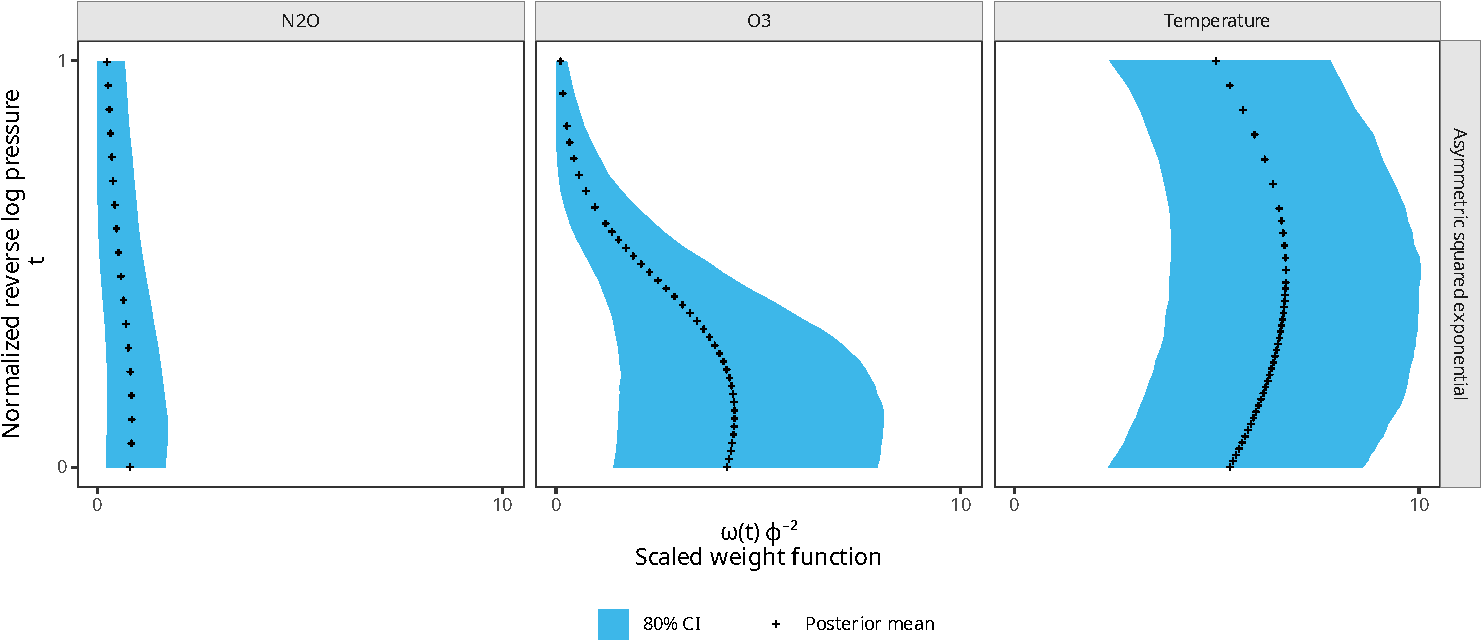
\includegraphics[width=\textwidth]{inc/mmls_weight_posterior_mini1}
          \label{fig:mmls-weight-posterior-mini1}
        \end{figure}
      \end{block}

      \begin{minipage}[t]{1.0\linewidth}
        \begin{minipage}[t]{.5\linewidth}
          \begin{block}{Which inputs are more relevant?}
            \begin{figure}
              \centering
              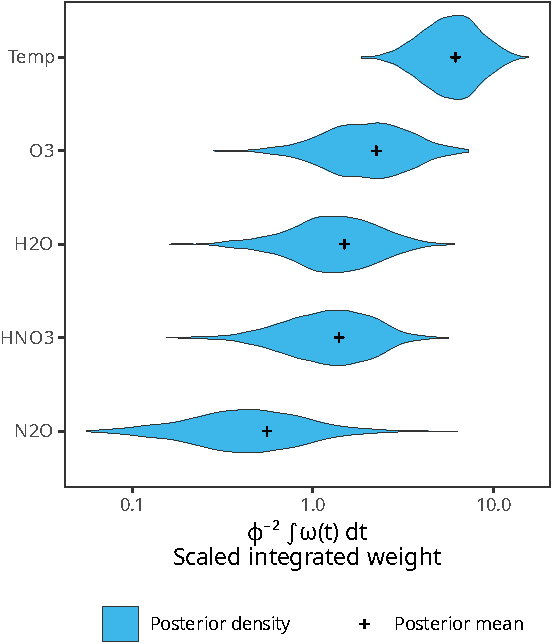
\includegraphics[width=\linewidth]{inc/mls_weight_integral.pdf}
            \end{figure}
          \end{block}
        \end{minipage}
        \begin{minipage}[t]{.5\linewidth}
          \begin{block}{Out-of-sample prediction}
            \begin{tblr}[evaluate=\fileInput]{
                width=\textwidth,
                colspec={Q[l,11ex]RRRRR},
                rows={font=\normalsize}}
              \fileInput{inc/mmls_validation_mean}
            \end{tblr}
          \end{block}
          \begin{block}{In summary...}
            \begin{itemize}
            \item Fewer parameters than a vector representation
            \item Better prediction than FPCA (information loss)
            \item Rich interpretation
            \item The weight posterior can feed downstream analysis (e.g.,
              calibration, design)
            \end{itemize}
          \end{block}
        \end{minipage}
      \end{minipage}
    \end{minipage}%
  }
  \colorbox{black}{
    \begin{minipage}[t][76cm][t]{3cm}
      %Padding
    \end{minipage}%
  }

  \begin{minipage}[t][5cm][t]{116cm}
    \textbf{Acknowledgements}. MLS team at Jet Propulsion
    Laboratory for their insight in the instrument, the forward model, and other
    relevant atmospheric science concepts.
    Partially funded by Iowa State University through the
    Presidential Interdisciplinary Research Initiative on C-CHANGE:~Science
    for a Changing Agriculture, and the Foundation for Food and Agriculture
    Research.
    % \textbf{References}.
    % \printbibliography[heading=none]{}
  \end{minipage}




  % \begin{columns}[t]


  %   \separatorcolumn{}







  % \separatorcolumn{}

  % %% Column 1 ------------------------------------------------------------------
  % \begin{column}{\colwidth}
  %   \begin{block}{Automatic Relevance Determination}
  %     $\mathrm{Cor}(y_i, y_j) = e^{-\theta {(x_i - x_j)}^2}$
  %     where $\theta\in\mathbb{R}^+$ is a weight driving the response correlation

  %     \begin{figure}
  %       \centering
  %       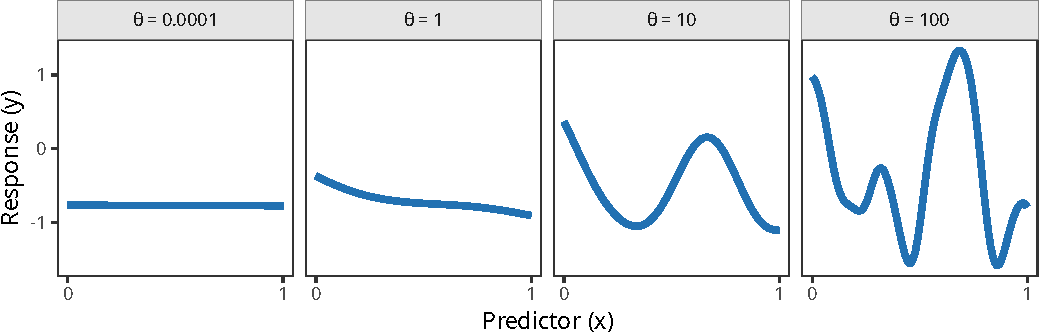
\includegraphics{inc/ard_response_profiles.pdf}
  %     \end{figure}
  %   \end{block}

  %   \begin{block}{Automatic Dynamic Relevance Determination}
  %     A framework for Gaussian Processes with functional inputs
  %     $X(t)\in\mathcal{X} = \left\{X:[0,1]\to\mathbb{R}\right\}$, $t\in[0, 1]$
  %     and a scalar output $y\in\mathbb{R}$. Let $f:\mathcal{X}\to\mathcal{Y}$ be
  %     an unknown function with evaluations $y_i = f(X_i)$, $i = 1, \dots,
  %     N\in\mathbb{N}$.
  %     \begin{align}
  %       \mathbf{y}
  %       &\sim \mathcal{N}\left(\mathbf{m}_f, \sigma_{f}^{2} \ \mathbf{R}_f
  %         + \sigma_{\varepsilon}^{2}\mathbf{I}\right) \\
  %       (\mathbf{m}_f)_i
  %       &= m_f(X_i) \\
  %       {\left(\mathbf{R}_f\right)}_{ij}
  %       &=
  %         \text{exp}\left\{
  %         -0.5 \phi^{-2} \ d_f(X_i, X_j)
  %         \right\}
  %       \\
  %       d_f(X_i, X_j)
  %       &= \int_{\mathcal{T}}
  %         \omega(t)
  %         {\left(X_i(t) - X_j(t) \right)}^2 dt
  %       \\
  %       \omega(t)
  %       &: \mathcal{T}\to\mathbb{R}^+
  %     \end{align}
  %     $\sigma_{\varepsilon}^2 > 0$,
  %     $\sigma_{f}^2 > 0$,
  %     $\phi > 0$,
  %     $i, j = 1, \dots, N$,
  %     and $m_f(\cdot)$ is a mean function left unspecified w.l.o.g.
  %   \end{block}

  %   \begin{block}{Choice of weight function}
  %     \begin{itemize}
  %     \item Learn how the input predictive relevance varies over the index
  %       space.
  %     \item Smoothness: Enforce smoothness on relevance over the index space.
  %     \item Parsimony: fewer parameters than the vector representation.
  %     \item Interpretation: for modeling feedback loop and understanding of the
  %       underlying physical model.
  %     \end{itemize}
  %   \end{block}

  %   \begin{block}{Input relevance statistics}
  %     \begin{column}{.4\linewidth}
  %       \begin{equation}
  %         \tau=\argmax_{t\in\mathcal{T}}\omega(t)
  %       \end{equation}
  %     \end{column}
  %     \begin{column}{.4\linewidth}
  %       \begin{equation}
  %         \Omega=\phi^{-2}\int_\mathcal{T}\omega(t)\,\mathrm{d}t
  %       \end{equation}
  %     \end{column}
  %   \end{block}

  %   \begin{block}{Learning \& validation}
  %     Fully Bayesian inference on the unknown quantities $\bm{\theta}$.
  %     One MCMC chain~\citep{raftery1992} with $M \in \mathbb{N}$ post warm-up
  %     samples generated via the NUTS algorithm~\citep{hoffman2014}.
  %     \begin{align}
  %       \label{eq:margina-likelihood}
  %       \log p(\mathbf{y} | \mathbf{X}, \bm{\theta})
  %       =& -\frac{1}{2}
  %          {(\mathbf{y} - \mathbf{m}_y)}^\top
  %          {\mathbf{S}_y}^{-1}
  %          {(\mathbf{y} - \mathbf{m}_y)}
  %          -\frac{1}{2}
  %          \log | \mathbf{S}_y |
  %          - \frac{n}{2} \log 2\pi \\
  %       \label{eq:parameter-posterior}
  %       \log p(\bm{\theta} | \mathbf{y}, \mathbf{X})
  %       \propto&
  %                \log p(\mathbf{y} | \mathbf{X}, \bm{\theta}) +
  %                \log p(\bm{\theta}).
  %     \end{align}

  %     Validation statistic posterior expectation approximated using a thinned
  %     posterior parameter sample with $\tilde{M} \in \mathbb{N}$ draws.
  %     \begin{align}
  %       \hat{v}_1
  %       &= {\tilde{M}}^{-1} \sum_{{\tilde{m}}=1}^{{\tilde{M}}} N^{-\frac{1}{2}} \norm{%
  %         \EE{\bm{y}_{*} | \bm{X}, \bm{X}_{*}, \bm{y}, {\bm{\theta}}_{{\tilde{m}}}} -
  %         \bm{y}_{*}
  %         } \label{eq:validation-rmse} \\
  %       \hat{v}_2
  %       &= {\tilde{M}}^{-1} \sum_{{\tilde{m}}=1}^{{\tilde{M}}}
  %         p(\bm{y}_{*} | \bm{X}, \bm{X}_{*}, \bm{y},
  %         {\bm{\theta}}_{{\tilde{m}}}) \label{eq:validation-ppld}
  %     \end{align}
  %   \end{block}
  % \end{column}

  % \separatorcolumn{}

  % %% Column 2 ------------------------------------------------------------------
  % \begin{column}{\colwidth}
  %   \begin{block}{Microwave Limb Sounder}

  %     \begin{itemize}
  %     \item Computer model: forward
  %       model~\cite{read2006,schwartz2006,waters2006} estimates, or
  %       \emph{retrieves}, geophysical variables from electromagnetic radiation
  %     \item Planetwide, daily data products~\cite{liversey2020} and uncertainty
  %       experiments~\cite{turmon2019,braverman2021} rely on a myriad of runs
  %     \item Output: score for reflected sunlight around 190GHz~\cite{johnson2020}
  %     \item Functional input: atmospheric profiles over a vertical grid
  %     \item We consider some species in pressure regions expected to be
  %       well-informed by the measurements~\cite{liversey2020}
  %     \end{itemize}

  %   \end{block}

  %   \begin{block}{Data}
  %     \begin{figure}
  %       \centering
  %       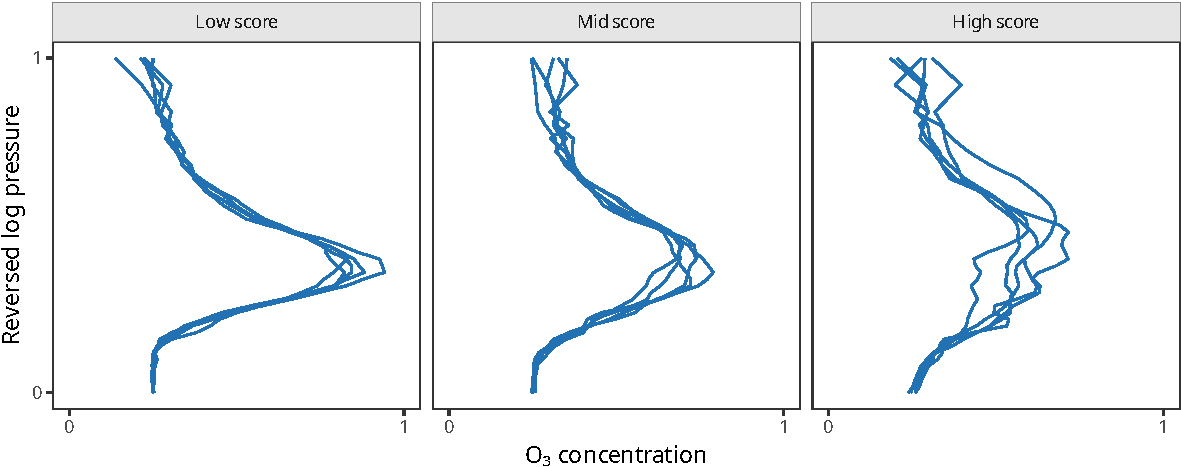
\includegraphics[width=\linewidth]{inc/mls_input_profiles}
  %     \end{figure}

  %     \begin{center}
  %       Radiance score variability seems associated with the tropopause Ozone
  %       concentration
  %     \end{center}
  %   \end{block}

  %   \begin{block}{Asymmetric Double Exponential weight function}
  %     \begin{figure}
  %       \centering
  %       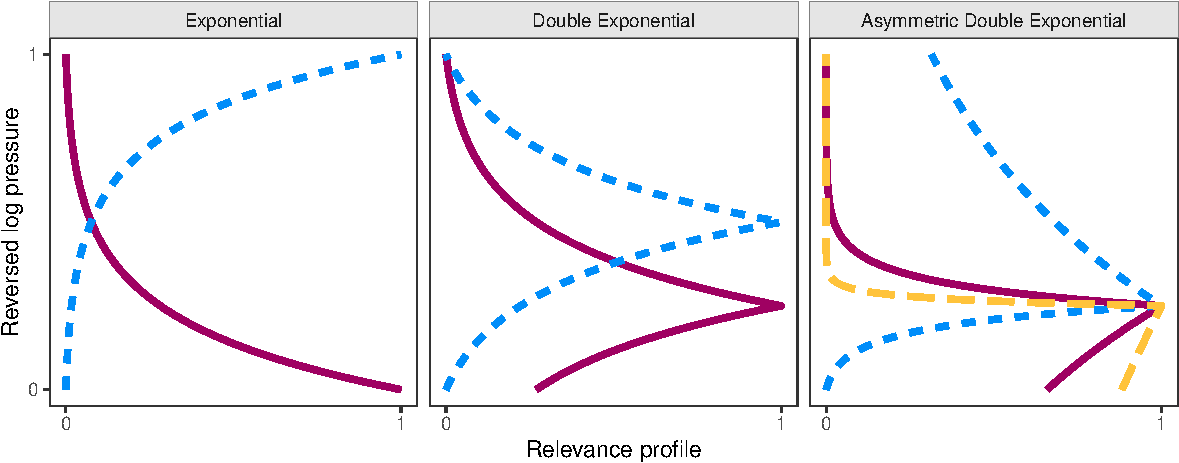
\includegraphics[width=\linewidth]{inc/mls_weight_profiles}
  %     \end{figure}

  %     \begin{equation}
  %       \omega(t)
  %       =
  %       \text{exp}\left\{-(t - \tau)\lambda\kappa^s s\right\}
  %     \end{equation}
  %     Space:
  %     $\omega(t): \mathcal{T} = [0, 1] \to (0, 1]$,
  %     $s = \text{sign}(t - \tau)$,
  %     $\tau\in[0,1]$,
  %     $\lambda > 0$,
  %     $\kappa > 0$ \\
  %     Priors:
  %     $\indent\tau \sim \textsc{Beta}$,
  %     $\lambda \sim \textsc{N}^{+}$,
  %     $\log(\kappa) \sim \textsc{N}$
  %   \end{block}


  %   \begin{block}{In which part of the atmosphere are the inputs most relevant?}
  %     \begin{figure}
  %       \centering
  %       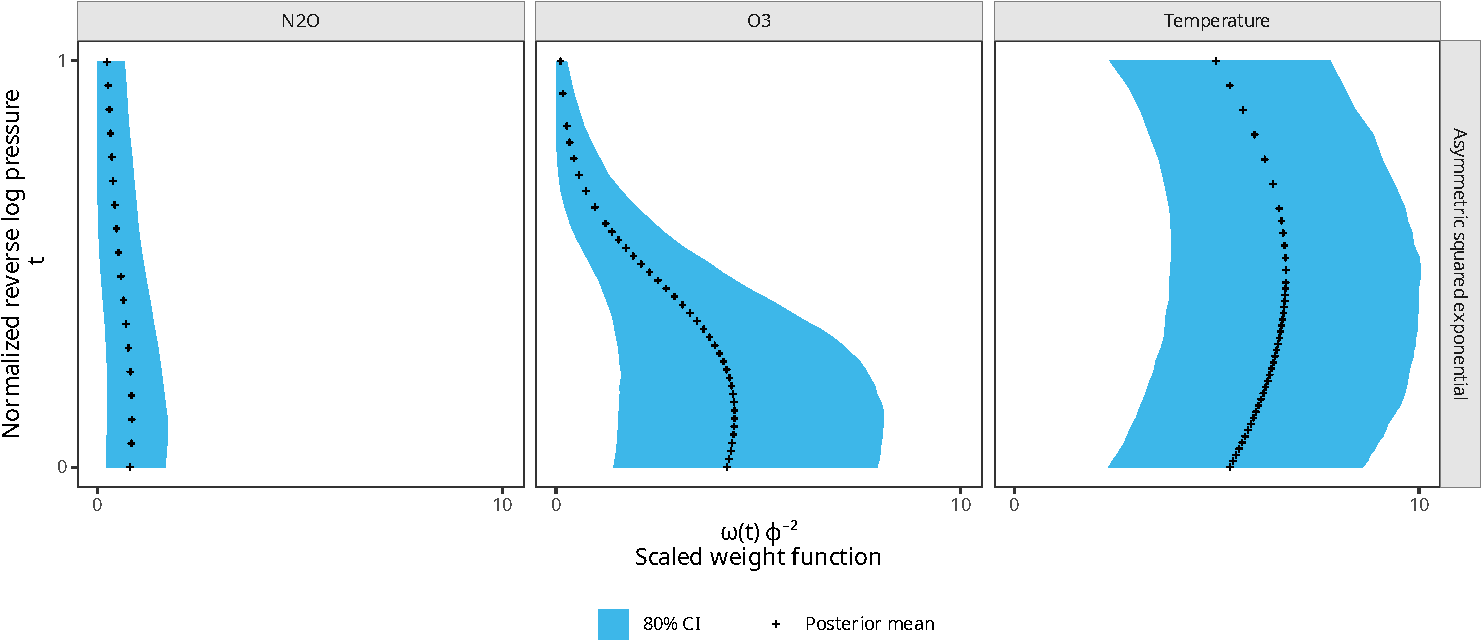
\includegraphics[width=\textwidth]{inc/mmls_weight_posterior_mini1}
  %       \label{fig:mmls-weight-posterior-mini1}
  %     \end{figure}
  %   \end{block}

  %   \begin{block}{Which inputs are more relevant?}
  %     \begin{figure}
  %       \centering
  %       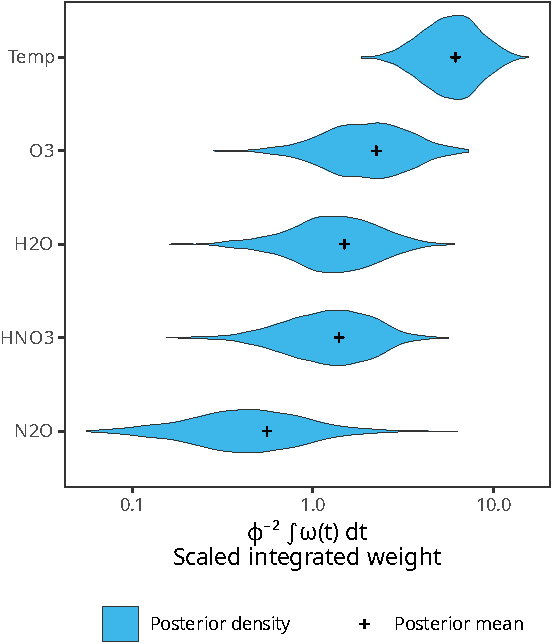
\includegraphics[width=\linewidth]{inc/mls_weight_integral.pdf}
  %     \end{figure}
  %   \end{block}
  % \end{column}

  % \separatorcolumn{}

  % % Column 3 -------------------------------------------------------------------
  % \begin{column}{\colwidth}
  %   \begin{block}{Water Erosion Prediction Project}
  %     \shortlipsum{}
  %   \end{block}
  % \end{column}

  % \separatorcolumn{}

  % % Column 4 -------------------------------------------------------------------
  % \begin{column}{\colwidth}
  %   \begin{block}{The rest goes here}
  %     \shortlipsum{}
  %   \end{block}
  % \end{column}

  % \separatorcolumn{}

  % % Blank padding to the right -------------------------------------------------
  % \vrule{}
  % \begin{column}{\padwidth}
  %   % padding
  % \end{column}

%\end{columns}
\end{frame}

\end{document}

%%% Local Variables:
%%% mode: latex
%%% TeX-master: t
%%% End:
